\chapter{Principy a historie regulárních výrazů}\label{sec:Principle}

Tato kapitola se zabývá definicí regulárních výrazů, jejich fungováním a jak se jednotlivé implementace mohu lišit. 
Součástí jejích implementace, provází několik pojmů z teoretické informatiky, odkud pocházejí.
Hlavně se jedná o \textbf{Konečné automaty} a \textbf{Thompsonovo sestrojení}.

\section{Formální jazyk}
Formální jazyk je libovolná množina konečných slov nad určitou abecedou \cite{MUNIFL}. 
Slova chápeme jako řetězce znaků, která jsou přijímaná zadaným jazykem.
Tato slova musí být sice konečná ale množina těchto slov může být nekonečná. 
Tyto jazyky mohou být definovány regulárními výrazy, formální gramatikou,
konečnými automaty a dalšími. Regulární jazyky jsou pak jednou z možných definic formálních jazyků. 

\section{Konečný automat}\label{sec:FiniteAutomaton}
Ve spojení s regulárními výrazy se často pojí konečné automaty, jedná se o další oblast z teoretické informatiky.
Tato práce implementuje regulární výrazy právě ve forme konečných automatů.
Zjednodušeně se dá říct, že konečný automat je model jednoduchého počítače, který má určitý počet stavů a přechodů \cite{Havrlant}. 

Stavy jsou typicky zakreslovány jako kružnice, a každý automat musí obsahovat alespoň jeden počáteční stav, ale může jich také obsahovat více. 
To stejné platí pro konečný/é stav/y. 
Konečné stavy se také vyznačují jako kruh, ale z dvojitou čárou. 
Počáteční stavy, jsou označovány jako stav, do kterého vede šipka, která ale nevychází z jiného stavu.
Přechody jsou pak šipky vedoucí z jednoho stavu do druhého a jsou označeny přechodovým symbolem.
Pro upřesnění, přechod může odkazovat na stejný stav ze kterého vychází.
Tyto přechody nám říkají, že pokud chceme přejít z jednoho stavu do druhého, tak musíme v přijímaném slově se posunout o přechodový symbol. 
Pokud to není možné, tak nelze přejít do tohoto stavu.

Konečné automaty se dělí na \textbf{deterministické} a \textbf{nedeterministické}, zkráceně \textbf{DKA} (deterministický konečný automat) a \textbf{NKA} (nedeterministický konečný automat).
DKA mohou mít v daném stavu pro každý znak abecedy \textbf{maximálně} jeden přechod, dále \textbf{nemohou} obsahovat tzv. prázdný znak často označovaný řeckým písmenem epsilon $\epsilon$.
Příklad tohoto automatu je možné vidět na obrázku~\ref{fig:DFAex}.
Naopak NKA umožňují jak prázdné znaky, tak více stejných přesunů z daného stavu. 
Prázdné znaky slouží pro změnu stavu bez změny aktuální pozice ve hledaném slově. 
Pro ukázku lze porovnat dva ekvivalentní konečné automaty,
NKA na obrázku~\ref{fig:NFAex} a DKA na obrázku~\ref{fig:DFAex}.
Na závěr lze podotknout, že každý NKA je možné převést na ekvivalentní DKA.

\begin{figure}[!h]
	\centering
	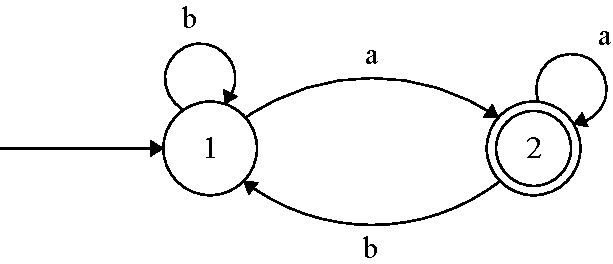
\includegraphics[width=0.45\textwidth]{Figures/DFA_example.pdf}
	\caption{Příklad deterministického automatu přijímající slova obsahující písmena z abecedy \{a, b\} končící písmenem a}
	\label{fig:DFAex}
\end{figure}

\begin{figure}[!h]
	\centering
	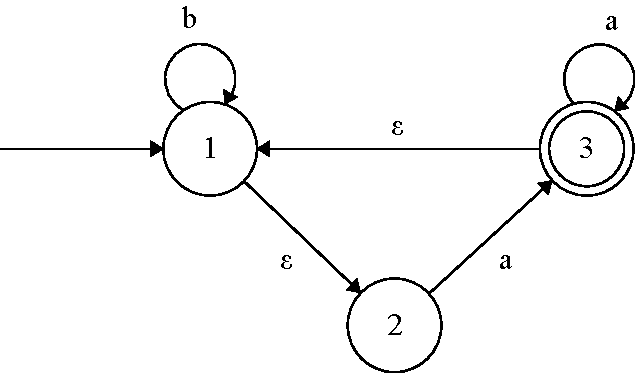
\includegraphics[width=0.45\textwidth]{Figures/NFA_example.pdf}
	\caption{Příklad nedeterministického automatu ekvivalentního k předchozímu deterministickému}
	\label{fig:NFAex}
\end{figure}

\section{Bezkontextová gramatika}
Součástí této práce je i využití Bezkontextové gramatiky, pro nadefinování syntaxe regulárních výrazů.

Bezkontextová gramatika, je jedna další z možných definic formálních jazyků. 
Je určená konečnou množinou \textbf{neterminálních symbolů} (proměnných), konečnou množinou \textbf{terminálních symbolů}, která nesmí mít žádné prvky společné s předchozí množinou.
Dále je součástí \textbf{počáteční neterminál}, s konečnou množinou \textbf{přepisových pravidel}\cite{MUNIFL}.

Pro příklad může sloužit výraz $A \longrightarrow \beta$, kde A je neterminál a $\beta$ je řetězec složený z terminálů a/nebo neterminálů. 
Dále šipka indikuje \textbf{přepsání} tzn. levá strana se přepisuje na stranu pravou.
Konečný řetězec generovaný danou gramatikou, je pouze tvořen terminálními symboly.
Aby mohl být řetězec přijímaný zadanou gramatikou, musí ho být schopná vygenerovat.

\section{Vznik, implementace a vzory}
Regulární výrazy byly poprvé nadefinovány Americkým matematikem \textbf{Stephan Cole Kleene}, jako regulární jazyky. 
Dále se aplikovali v teoretické informatice, jako podkategorie \textbf{teorie automatů} a součást \textbf{formálních jazyků}.
Ačkoliv byly nadefinovány začátkem padesátých let, tak jejich využití v počítačích nastalo až na konci šedesátých let a to v 
jedním z nejznámějších operačních systémů UNIX.

\subsection*{Thompsonovo sestrojení}

První kdo navrhl implementaci používanou v počítačích byl \textbf{Ken Thompson}.
Principem byl převod regulárního výrazu na NKA.
Tato metoda se často používá doposud, v podobné či nezměněné podobě.
Algoritmus se pojmenoval \textbf{Thompson's construction} (Thompsonovo sestrojení), který převádí textovou reprezentaci výrazu na ekvivalentní nedeterministický automat.
Toto sestrojení je využito v této práci a blíže jej popisuje následující část textu.

NKA se běžně využívá, jelikož je poměrně jednoduchý na implementaci.
Také oproti DKA využívá \textbf{zpětného krokování} (backtracking) a povoluje složitější operace jako je \textit{rozhlédnutí se kolem sebe} (look-around).
Backtracking je důležitý pro NKA, jelikož neexistuje jednoznačná cesta vyhodnocení.
To znamená že, pokud je NKA ve stavu, ze kterého nelze pokračovat dále, tak je potřeba se vrátit do předchozího stavu.
DKA mají výhodu že jsou rychlejší, ale jsou typicky mnohem větší než jejich ekvivalentní NKA a neumožňují lehce implementovat některé složitější operace.
Také nepotřebují zpětné krokování, jelikož jejich cesta je deterministická tzn. existuje vždy jen jedna cesta pro hledané slovo.
Dnes se ale často využívá kombinace DKA i NKA, kdy DKA se využije pro rychlé vyhledání daného slova a pokud bylo slovo nalezeno, 
tak se použije NKA pro jejich rozšířené možnosti.

Výsledný NKA po Thompsonově sestrojení má právě jeden vstupní a výstupní stav. 
Thompsonovo sestrojení dále definuje několik následujících pravidel.

Prázdný výraz \textit{$\epsilon$}, je převedený na vstupní stav, přechod \textit{$\epsilon$} a konečný stav.
Výsledný konečný automat je na obrázku~\ref{fig:NFAepsilon}.
\begin{figure}[!h]
	\centering
	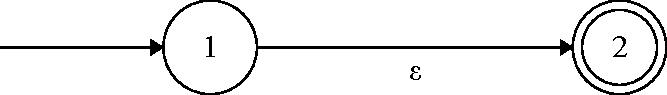
\includegraphics[width=0.5\textwidth]{Figures/NFA_epsilon.pdf}
	\caption{Převedený prázdný výraz \textbf{$\epsilon$}}
	\label{fig:NFAepsilon}
\end{figure}

Výraz \textit{a}, je převedený podobně jako prázdný výraz, ale s rozdílem přechodu \textit{a} místo \textit{$\epsilon$}.
Konečný automat, který tímto převodem vznikne je ukázán na obrázku~\ref{fig:NFAa}.
\begin{figure}[!h]
	\centering
	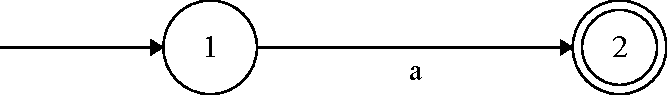
\includegraphics[width=0.5\textwidth]{Figures/NFA_a.pdf}
	\caption{Převedený výraz \textbf{a}}
	\label{fig:NFAa}
\end{figure}

Pro zadaný výraz \textbf{s|t} (varianta), kde \textit{s} je levá strana varianty a \textit{t} je pravá strana varianty, platí že ze stavu \textit{q} (počáteční stav) vedou dva přechody
\textit{$\epsilon$}, na počáteční stavy variant \textit{s} a \textit{t}. 
Z těchto počátečních stavů dále pokračuje sekvence stavů \textit{N(s)} pro \textit{s} a \textit{N(t)} pro \textit{t}.
Konce variant \textit{s} a \textit{t} mají každé jediný přechod \textit{$\epsilon$} na konečný stav \textit{f}.
Na obrázku~\ref{fig:NFAunion} je znázorněný výsledný NKA, kde skupina stavů v zelené části je \textit{s} a červená skupina je \textit{t}.
\begin{figure}[!h]
	\centering
	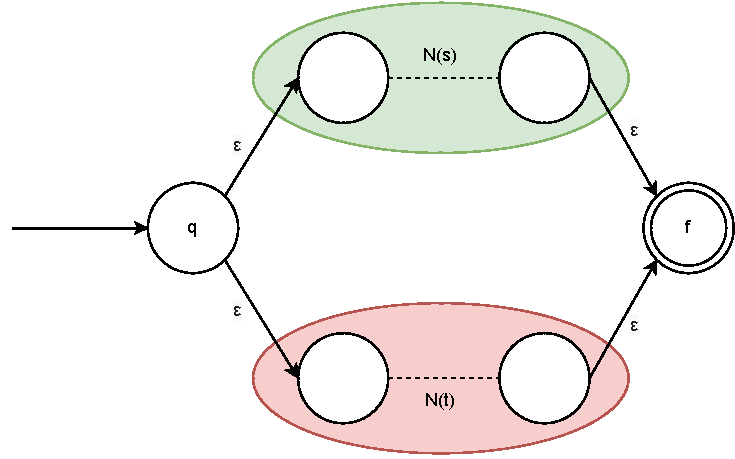
\includegraphics[width=0.6\textwidth]{Figures/NFA_union.pdf}
	\caption{Převedený výraz \textbf{s|t}}
	\label{fig:NFAunion}
\end{figure}

Další pravidla pro sestrojení lze například najít, v následujících článcích \cite{Thompson1,Thompson2}.
Některé pravidla, jsou v této práci upravená, ale fungují na stejném principu.

\subsection*{Základní vzory regulárních výrazů}
V Předchozích sekcích, již byly popsány základní konstrukce týkající se regulárních výrazů.
Tato sekce se zabývá jejich základními vzory, nebo-li jejich formou zápisu a syntaxí.

Za nejjednodušší výraz lze považovat prázdný výraz, také označovaný jako $\epsilon$. 
Tento výraz dokáže přijímat slova délky 0 resp. prázdné slova.
Výrazy mohou obsahovat \textbf{téměř} libovolný znak, který bude přijímat slova s tímto znakem. 
Avšak nemohou být použity znaky, které jsou rezervované, nebo-li jsou součástí syntaxe regulárních výrazů.
Chceme-li použít tyto znaky je potřeba použít zpětné lomítko \textbackslash. 
Takové spojení znaku a zpětného lomítka se pak anglicky nazývá \textbf{escaped character}.
Ačkoliv také existují znaky, které nejsou součástí rezervovaných znaků, ale lze před nimi použít zpětné lomítko.
Funkcionalita těchto znaků se následně mění. 
Například pokud použijeme zpětné lomítko před znakem \textit{d}, tak to ve výrazu značí přijmutí čísla od 0 do 9.

Iterace, je možnost jak lze opakovaně provádět nějaký vzor.
Například lze iterovat znak, skupinu a další konstrukce. 
Nelze však opakovat jakýkoliv vzor.
Prvním typem iterace je \textbf{*}, známa jako \textbf{Kleene star}.
Tento druh iterace, může mít počet opakování od \textbf{0} do \textbf{n}. 
Dále existují další 2 typy iterací, a to je iterace v rozmezí $1-n$ označována znakem + a \textit{iterace v rozmezí}, která se značí \{od,do\}.

Operace \textit{výběr}, je dalším základním vzorem pro regulární výrazy. 
Jedná se o výběr mezi pravou a levou stranou. 
Oddělovacím znakem je typicky | podobně jako bitová operace \textit{OR} v mnoha programovacích jazycích.

Dalšími základními konstrukty jsou například skupiny, které jsou obaleny v jednoduchých závorkách.
Ty slouží k rozdělení částí regulárních výrazů, které jsou po dokončení vyhledávání, přístupné jako oddělené části vyhledání.

Na obrázku \ref{fig:REGEXEXMP} lze vidět příklad regulárního výrazu, ve kterém jsou použity a popsány některé ze zmíněných vzorů.

\begin{figure}[!h]
	\centering
	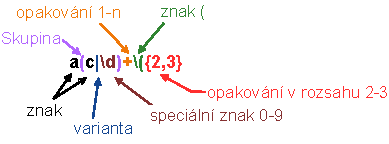
\includegraphics[width=0.5\textwidth]{Figures/regex_exmp.pdf}
	\caption{Příklad regulárního výrazu}
	\label{fig:REGEXEXMP}
\end{figure}

\subsection*{Implementace v programovacích jazycích}\label{sec:impipl}

V dnešní době mají v podstatě skoro všechny programovací jazyky, nějakou formou implementované regulární výrazy.
Tato implementace se však často liší. 
Sice jejich základ bývá stejný, ale co se týče obsáhlosti a syntaxe se často liší.
Může se tak stát to, že funkcionalita podporována jedním jazykem, není podporovana druhým.
Taktéž oproti původním regulárním výrazům, dnešní implementace obsahují mnohdy složitější koncepce, jako je look-around, nebo například rekurze.
Někdy jazyky sice sdílí stejné konstrukce, ale mohou se lišit syntaxí.

Look-around je již celkem pokročilá funkcionalita, jejímž principem je, takzvané nezachytávání znaků při zpracovávání.
Typicky je dělíme podle směru a to na \textit{dopředné} a \textit{zpětné}.
Pak je dělíme podle podmínění a to na \textit{kladné} a \textit{negativní}.
Pokud máme kladné podmínění \textbf{musí} uzavřený výraz být splněný a pokud máme záporné tak \textbf{nesmí} být splněný.
V původní formě regulárních výrazů, tato funkce neexistovala.

Mnohdy je potřeba, nalezený řetězec rozdělit do skupin. 
Tuto možnost dnešní implementace také umožňují.
Chceme-li zdůraznit že zadaný podvýraz je skupinou, obalíme ho do závorek.
Tato vlastnost je důležitá, jelikož není potřeba v již nalezeném řetězci, hledat další podřetězce pomocí dalšího výrazu.
Skupiny se dělí na zachytávající (capturing), pojmenované (named) a nezachytávající (non-capturing).
Pojmenované patří pod zachytávající, akorát jsou identifikovány pomocí názvu místo indexu.
Obě skupiny zůstávají zachycené po dokončeném vyhledávání.
Nezachytávající skupiny slouží čistě pro regulární výrazy, například při opakování části výrazu, ale ve výsledku se již nenachází.

Asi nejobsáhlejší implementací je \textit{PCRE} (Perl-Compatible Regular Expressions) a \textit{PCRE2}.
Tento standard pochází z jazyka Perl, ale také je například součástí jazyka PHP.
Nachází se zde již poměrně složité vzory, jako jsou podmínky, nebo rekurze.

\endinput

%TODO: popsat blíže rozložení na DKA a proč to není praktické